\documentclass[runningheads]{llncs}

\usepackage[T1]{fontenc}
\usepackage{graphicx}
\usepackage{booktabs}

\begin{document}
    \title{Data-Driven Approaches for Identifying Depression Severity in Social Media Posts}
    \titlerunning{Data-Driven Identification of Depression Severity}

    \author{Paul-Adrian Uif\u{a}lean}
    \authorrunning{Paul Uif\u{a}lean}

    \institute {Babe\c{s}-Bolyai University \\ \email{paul.uifalean@stud.ubbcluj.ro}}
    
    \maketitle 
    
    \begin{abstract}
        In this study, I explored different approaches to classify depression severity from social media text. I combined multiple publicly available datasets to build a unique dataset labeled with three severity levels: not depression, moderate, and severe. I evaluated traditional machine learning models using TF-IDF and sentence embeddings, deep learning models based on BiLSTM with pre-trained GloVe embeddings, and a fine-tuned DistilBERT transformer model, pre-trained with masked language modeling. My results show that simple traditional models with strong features perform best, while deep learning models faced challenges likely due to limited and imbalanced data. The DistilBERT model performed competitively but requires more fine-tuning and data augmentation to reach its full potential. I conclude that, given current data constraints, simpler models remain strong baselines, and future work should focus on collecting richer data and improving augmentation and fine-tuning methods for advanced models.
    \end{abstract}
    
    \keywords{Depression Severity, Data Augmentation, Sentence Embeddings, Class Imbalance, GloVe Embeddings, Masked Language Modeling, Transformer Fine-Tuning}

    \section{Introduction}

The task of processing natural language continues to grow in both importance and popularity among researchers, but everyday users as well, driven by the rapid rise of large language models and the ongoing changes towards a more semantic web. Technologies such as knowledge graphs and contextual embeddings are becoming more essential in the interpretation of human language for machines, as more and more of the web needs to be machine-readable. This area of artificial intelligence stands out due to its direct interaction with users, who not only benefit from its applications, but also contribute to its improvement through feedback and the data they generate.

In recent years, there has been growing interest in using NLP to support mental health analysis, particularly through the examination of social media and online forums. These platforms often serve as safe spaces where people express their thoughts, emotions, and struggles, including experiences related to depression. While identifying whether a post reflects depression is already a complex task, understanding how severe that depression might be is even more of a challenge.

This research addresses the open challenge posed by the RANLP 2025 shared task: Identification of the Severity of Depression in Forum Posts.

The primary research question of this study is to evaluate various feature representations and modeling approaches for improving the identification of depression severity in texts. Specifically, I compare traditional feature extraction methods like TF-IDF with advanced sentence transformer embeddings to understand their relative effectiveness. I also examine the impact of different pre-trained word embeddings, comparing general-domain GloVe vectors to Twitter-specific embeddings within BiLSTM architectures. Finally, I investigate the benefits of domain-adaptive pre-training using masked language modeling on DistilBERT, followed by fine-tuning, to explore how large language models can enhance performance on this specialized task.

In addition to exploring various modeling techniques, with this research I place strong emphasis on data-level experimentation. Rather than using a single dataset, I attempted to construct a comprehensive dataset by merging and standardizing multiple publicly available depression-related corpora. With this I aimed to increase both the volume and diversity of data, helping to improve representation across different severity levels. To further address class imbalances, I applied resampling methods such as minority class oversampling. Additionally, I explored straightforward data augmentation techniques, including synonym replacement to synthetically expand the training set and enhance model generalization.

The content of this research paper is organized as follows: the Related Work section provides an overview of prior research relevant to this study. The Data section describes the dataset preparation, including cleaning and analysis steps. The Methodology section explains the approaches and configurations used throughout the experiments. The Results section presents the experimental findings and compares the performance of different models. Finally, the Conclusion summarizes the key insights and discusses their broader implications.
    \section{Related Work}

In this section, I review relevant studies that motivate the current research. Prior work on detecting signs of depression from text-based social media posts can be grouped into three main areas: dataset construction and annotation, machine learning and deep learning methodologies, and the use of contextualized language models.

Recent research on detecting signs of depression from social media highlight both the difficulties and opportunities for applying NLP in mental health analysis. A fundamental contribution in this area is presented in \cite{Kayalvizhi_2022_Dataset}. In this work, the authors emphasize the importance of carefully curated data for effective depression detection. They create a labeled dataset by extracting and manually annotating posts from social media platforms, categorizing them into different severity levels of depression based on psycholinguistic indicators. Their analysis revealed distinct language patterns that relate to mental health states. This study addressed a significant gap in annotated resources and provided early performance benchmarks with classic machine learning models such as SVMs and Naive Bayes, which showed moderate success in identifying severity levels.

Following this, the same authors organized a shared task to encourage wider research on this problem \cite{Kayalvizhi_2022_Findings}. Participants used a variety of methods, ranging from traditional feature-based models to more advanced deep learning architectures like LSTMs and transformers. The results showed that deep learning models, especially those fine-tuned on data from the depression domain, achieved better accuracy and F1 scores compared to traditional techniques.

Another significant contribution to the field comes from \cite{Poswiata_2022}, who participated in the LT-EDI shared task with their system. Their work centers on the use of RoBERTa, a highly optimized BERT-based language model, which they fine-tuned specifically for the detection of depressive signals in social media text. Their approach highlighted the benefits of transfer learning: by first training on large general datasets and then fine-tuning on depression-related texts, their model was able to adapt general language knowledge to this challenging and sensitive task. Their system ranked among the top performers in the shared task, showing how pretrained language models, when carefully fine-tuned can outperform other traditional methods for text that contains subtle psychological indicators.

\cite{Naseem_2022} introduced a framework for identifying depression severity on Reddit, emphasizing the importance of moving beyond binary classification by modeling depression as an ordinal task based on clinical standards like the Beck Depression Inventory (BDI). Their approach involved creating a new dataset labeled with four severity levels and developing a hierarchical attention mechanism to capture the progression and intensity of depressive symptoms. By testing on both a public multi-post dataset and a newly collected single-post dataset, their model showed improved accuracy and early detection over existing baselines.

Another notable contribution to depression severity detection comes from \cite{Munoz_2023}, who propose a balanced approach that prioritizes both interpretability and performance through a feature-based framework enhanced with distributional representations. Their work addresses two key limitations of deep learning models: high computational demands and limited transparency. While transformer-based models like BERT often achieve high accuracy, they are resource-intensive and operate as black boxes. In contrast, the authors offer a more scalable and interpretable solution by combining handcrafted linguistic, emotional, and cognitive features with distributional word embeddings, which enables decent performance in resource-constrained or more practical settings.
    \section{Data}

The dataset used in this study was constructed by aggregating and preprocessing multiple publicly available depression-related social media corpora. The goal was to produce a unified, high-quality dataset suitable for training and evaluating machine learning models tasked with detecting depression severity levels in textual content. This section outlines the origin, preparation, and final composition of the dataset used throughout my experimentation. I selected two primary sources of data:

The first is the DEPSEV dataset, which contains user-generated posts annotated according to clinically derived categories of depression severity, such as minimum, mild, and severe. It provides structured and medically grounded labels for identifying levels of depressive symptoms in text.

The second is the DEPSIGN dataset, which is a combination of three related smaller datasets, referred to as DEPSIGN\_1, DEPSIGN\_2, and DEPSIGN\_3. Each of these subsets contains text posts labeled for signs of depression, albeit using slightly different taxonomies and conventions, which I addressed during data cleaning and preprocessing. These datasets were first loaded independently and subjected to standardized cleaning procedures. Afterward, they were merged into a single corpus. Subsequently, this corpus was concatenated with the cleaned DEPSEV dataset to form the final dataset, which I refer to as DEPSET.

In order to ensure that all datasets are compatible and share a uniform common schema, I implemented several cleaning utilities, which include the process of converting all column names to lowercase and replacing all white spaces to underscore. Because every dataset had small differences in the labeling and text names, I needed to normalize them, so I identified every column that contains the "label" or "text" substrings in any format and standardized them accordingly. As a final initial cleaning step, I removed all columns which contained ID values, since these offer no value to the research, other than for ordering purposes.

The original label schema in the DEPSEV dataset contained four labels, and the lowest severity level was "minimum", whereas the other datasets included a label that indicated no depression levels at all. To align DEPSEV with the other datasets and to provide a clearer semantic interpretation, I applied a series of mappings: I relabeled "minimum" to a non-depression severity level and "mild" to "moderate". These adjustments produced a harmonized label taxonomy comprising of three category labels: not depression, moderate and severe. Of course, before deciding to remap those labels, I manually checked some of the minimum labeled texts. These mostly included neutral texts like advertising or casual conversations, which offer no real value being labeled as minimum.

After the merge into the final dataset, I applied several final cleaning steps. I began by checking for null values, which surprisingly were none. However, it appeared that there was a significant number of duplicate values among the DEPSIGN datasets. Initially I believed this to be an error, possibly the function misinterpreting similar text as duplicates, but after a thorough check through some duplicate data samples, I found that the texts were indeed one-to-one duplicates, so I removed them to prevent useless noisy data.

As a final step of data analysis, I performed a final verification on label frequency to assess class imbalance and data size. The final label distribution is shown in Table 1, below:

\begin{table}
    \centering
    \caption{Label distribution across datasets before and after merging}
    \begin{tabular}{lccc}
        \toprule
            \textbf{Dataset}        & 
            \textbf{Not Depression} & 
            \textbf{Moderate}       & 
            \textbf{Severe}         \\
        \midrule
            DEPSEV        & 2,587  & 684   & 282  \\
            DEPSIGN\_1    & 1,830  & 2,306 & 360  \\
            DEPSIGN\_2    & 848    & 2,169 & 228  \\
            DEPSIGN\_3    & 1,971  & 6,019 & 901  \\
        \midrule
            \textbf{Final Dataset} & 
            \textbf{6,112}         & 
            \textbf{6,438}         & 
            \textbf{1,218}         \\
        \bottomrule
    \end{tabular}
    \label{Table_1}
\end{table}

Even though the dataset seems clearly imbalanced, the severe class being misrepresented, I believe that this is more similar to a real-world scenario. Thankfully, the severe cases of depression are minimal in the real world or on the other hand, they may be less likely to be explicitly shared on public platforms. In order to combat the class imbalance, I implemented a few data-level solutions like oversampling and data augmentation, which I will cover in the next chapter in detail.

After data cleaning, I implemented a classic preprocessing function, which applies a sequence of operations, including: converting all text to lowercase, removing spaces, expanding words into their full form using contractions, the removal of URLs and HTML tags, and handling punctuation and extra unnecessary spaces.

Another piece of data that I used for this project is the Reddit Depression Corpora, a corpus which consists of 396,968 social media posts, gathered from various subreddits related to mental health, which I have used for pre-training DistilBERT using masked language modeling.

The main issue that I encountered while attempting to collect such data for the construction of a dataset was the sensitive and personal nature of the data. High-quality clinical data annotated by professionals in this domain is often protected by privacy regulations, which makes it difficult and unethical to share publicly. As a result, I relied on publicly available social media content, which, while accessible, may contain exaggerated, sarcastic or fabricated narratives, which can introduce noise into the dataset and potentially mislead and confuse machine learning models.

    \section{Methodology}

In this chapter, I will explain the methodology used in this research to build and evaluate depression severity classifiers. It includes some final data preparation steps such as label encoding, sampling and data augmentation strategies, describes the pipelines used for model training and evaluation strategies.

To begin the modeling process, I divided the final dataset into train and test subsets, with a split ratio of 80 to 20. Given the small amount of data, I experimented with a 70-30 split initially, but the differences between the splits were insignificant.

Since this task is multi-label classification instead of binary, I used the label encoder from the Scikit-learn library to encode string class labels into integer format. The encoder was then fit on the training labels and then applied to both training and test labels for consistency.

For evaluating model performance, I used a 5-fold cross-validation using StratifiedKFold. This approach is quite standard, but it is especially important to preserve the relative frequency of each class in every fold, given the class imbalance in my dataset. Similarly, I experimented with a 10-fold cross-validation, but the differences were minimal.

The first operation that I implemented to mitigate the impact of class imbalance was to compute class weights. I then applied those class weights to all compatible classifiers to adjust the learning process so that underrepresented classes receive proportionally more attention.

\subsection{Machine Learning Methodology}

In this part of the research, I evaluated both traditional machine learning models and sentence embedding-based classifiers, using two types of feature representations: Term Frequency-Inverse Document Frequency (TF-IDF) vectors and sentence embeddings. My previous research in this domain concluded that TF-IDF is superior to the Bag-of-Words(BoW) approach, so I chose this as traditional feature representation.

I configured the TF-IDF vectorizer to use unigrams and bigrams with a maximum of 5,000 features and filtered out the extreme common and rare terms to reduce noise. For the sentence embeddings, I utilized the all-MiniLM-L6-v2 model to compute dense vector embeddings of the input text. This approach should capture contextual and semantic relationships better than sparse representations.

The initial performances of the models were very poor, so I experimented with SMOTE (Synthetic Minority Oversampling Technique) to oversample the minority class in the training set. I applied SMOTE separately to both TF-IDF and embedding-based features.

I tested and evaluated three traditional classifiers across both feature types: Logistic Regression, Linear SVM and Random Forest. Each model was trained with the computed class weights and validated using the cross-validation strategy I mentioned earlier. For each model, I computed cross-validation scores and confusion matrices, and the main evaluation metrics are accuracy, F1 score, recall and precision, all weighted by class frequency.

After applying cross-validation, I compared all models based on their average performance across folds. The best-performing model will be re-trained on the full training set and evaluated on the testing set. 

\subsection{Deep Learning Methodology}

For the next component of my research, I implemented a Bidirectional Long Short-Term Memory (BiLSTM) neural network, enriched with two kinds of pre-trained GloVe embeddings that capture semantic meaning: general-domain embeddings and twitter-domain embeddings. My goal is to find out if the twitter-based embeddings will outperform the general-domain ones, given that they are trained specifically on social media texts, similar to my classification task.

I began by performing some data augmentation operations to further address the class imbalance. I applied a synonym-replacement augmentation approach using the nlpaug library with the SynonymAug augmenter configured with WordNet as the source. Each sample from the severe class was augmented with four additional variants, which boosted the minority class size. The original training size was 11,014 samples. The augmenter provided an additional 3,896 severe samples which produced 14,910 total training size post-augmentation.

After augmentation, I re-encoded the target labels and transformed them into categorical one-hot representations using TensorFlow, in order to make them compatible with the multi-class softmax output layer used in the neural networks.

The text sequences were tokenized with a vocabulary size limit of 10,000 and padded to a fixed maximum length of 100 tokens. I then mapped the 100-dimensional GloVe vectors to the tokenized vocabulary to create two embedding matrices, which I used as non-static input layers in their respective models.

I customized the model architecture as BiLSTM to capture both past and future temporal dependencies in the token sequences. The model layer architecture can be found in the figure below.

\begin{figure}
    \centering
    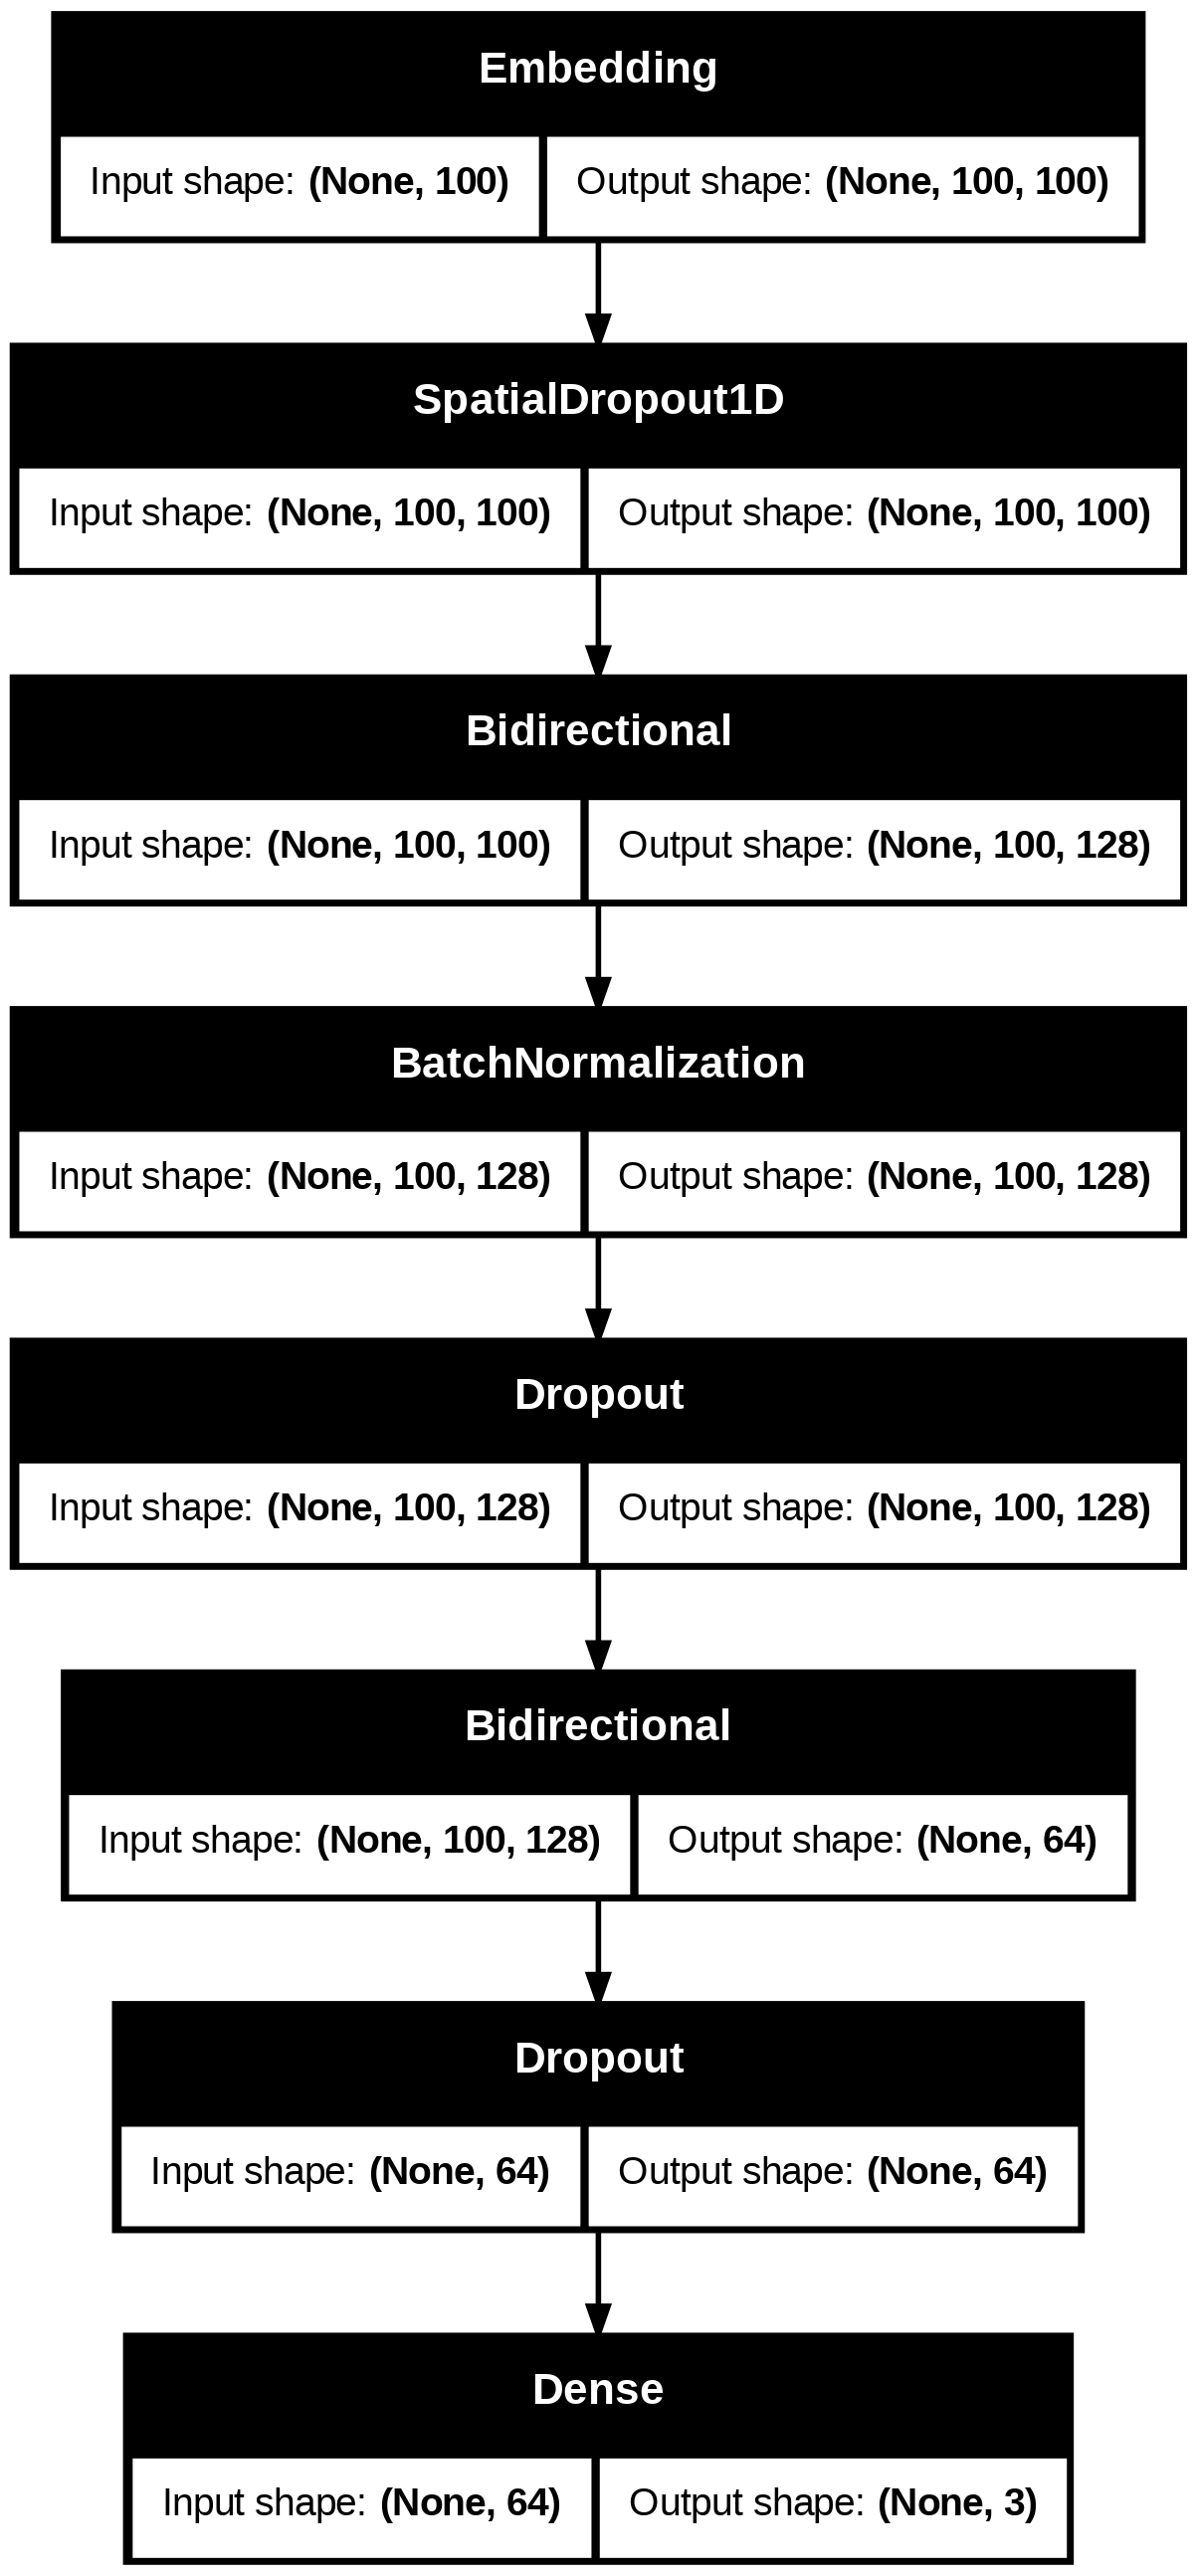
\includegraphics[width=0.5\linewidth]{img/model-architecture.png}
    \caption{BiLSTM Model Layer Architecture}
    \label{Fig_1}
\end{figure}

The initial Embedding layer is initialized with the appropriate pre-trained GloVe embedding and converts each token into a 100-dimensions vector. I also allowed for fine-tuning during training by specifying trainable weights.

I then used a Spatial Dropout layer of 0.2 to randomly drop entire embeddings, instead of individual features, in the hope of helping the model to generalize better.

Following that, I applied the first Bidirectional LSTM layer with 64 units to capture context in both forward and backward directions. This should enable the model to understand both preceding and succeeding context in sentences.

Initial training experiments were unstable, so I added a Batch Normalization layer that normalizes intermediate outputs and stabilizes training.

In order to help with generalization and prevent overfitting I also used three separate Dropout layers, with a rate of 0.2 and 0.5 respectively.

A second BiLSTM layer with 32 units was stacked next to allow the model to refine learned representations with additional processing.

The final layer is a standard Dense layer with a softmax activation and three output units, which corresponds to my three severity labels.

Each model was compiled with the Adam optimizer and trained using categorical cross-entropy loss. I implemented an early stopping callback to prevent overfitting based on a validation loss, with a patience of 3 epochs. I also applied the class weights from the original label distribution.

I trained each model up to 20 epochs with a batch size of 512 and then evaluated them on the test set using the classification metrics defined at the beginning of this chapter.

\subsection{LLM-based Methodology}

Another goal of this research is to compare the effectiveness of Large Language Models (LLMs) with traditional machine learning and deep learning models. For this, I implemented a two-stage transfer learning approach using DistilBERT.

I began by pre-training a DistilBERT model on an unlabeled corpus using Masked Language Modeling. This step aimed to adapt the general-purpose language model to the specific linguistic pattern found in my domain-related corpus. I used the uncased base version and trained for 3 epochs with a masked token probability of 15\% using the Trainer API from HuggingFace Transformers library.

After pre-training, I reused the masked language model to initialize DistilBERT for sequence classification with three output labels corresponding to my severity classes. I used for both steps the fast tokenizer with a maximum length of 128 tokens.

Finally, I fine-tuned the classification model using supervised learning for 6 epochs. I configured the training with a learning rate of $2 \times 10^{-5}$, a batch size of 32 and weight decay of 0.01.

After fine-tuning, I evaluated the model using custom metrics, including accuracy, precision, recall and F1-score.
    \section{Results}

This chapter presents the results of the classification models that I developed. I focus on comparing the performance of traditional machine learning models, deep learning architectures, and a fine-tuned Large Language Model (DistilBERT) in detecting depression severity across three classes: not depression, moderate, and severe. I evaluated all models using accuracy, F1-score, precision, and recall, with results weighted by class frequencies. Additionally, I also examined confusion matrices to gain insight into class-wise predictions.

\subsection{Machine Learning Models Results}

Table \ref{Table_2} summarizes the performance of traditional machine learning models across two types of feature representations: TF-IDF and sentence embeddings. Among the TF-IDF-based models, the Random Forest classifier achieved the best overall results, with an accuracy of 74.4\% and an F1-score of 74.8\%. It outperformed both Logistic Regression and Linear SVC, which indicates its ability to capture complex feature interactions.

\begin{table}
    \centering
    \caption{Performance of Machine Learning Models}
    \label{Table_2}
    \begin{tabular}{ccccc}
        \toprule
            \textbf{Model}          & 
            \textbf{Accuracy (\%)}  & 
            \textbf{F1 Score (\%)}  & 
            \textbf{Recall (\%)}    & 
            \textbf{Precision (\%)} \\
        \midrule
            Logistic Regression (TF-IDF)      & 67.1 & 65.1 & 67.1 & 68.2 \\
            Linear SVC (TF-IDF)               & 71.8 & 70.7 & 71.8 & 70.9 \\
            Random Forest (TF-IDF)            & 74.4 & 74.8 & 74.4 & 75.4 \\
        \midrule
            Logistic Regression (Embeddings)  & 57.3 & 53.2 & 57.3 & 61.5 \\
            Linear SVC (Embeddings)           & 60.5 & 57.8 & 60.5 & 62.6 \\
            Random Forest (Embeddings)        & 76.3 & 76.4 & 76.3 & 76.6 \\
        \bottomrule
    \end{tabular}
\end{table}

Interestingly, while TF-IDF-based models generally outperformed their embedding-based counterparts, the Random Forest model using sentence embeddings achieved the highest performance across all traditional models, with an accuracy of 76.3\% and an F1-score of 76.4\%. This suggests that Random Forests may be more capable of leveraging the dense semantic information encoded in embeddings compared to linear models.

The confusion matrices for each model, shown in Figure \ref{Fig_2} provide additional insights. The Random Forest (Embeddings) model showed improved classification of the severe class compared to others, which is notable given the severe class imbalance.

\begin{figure}
    \centering
    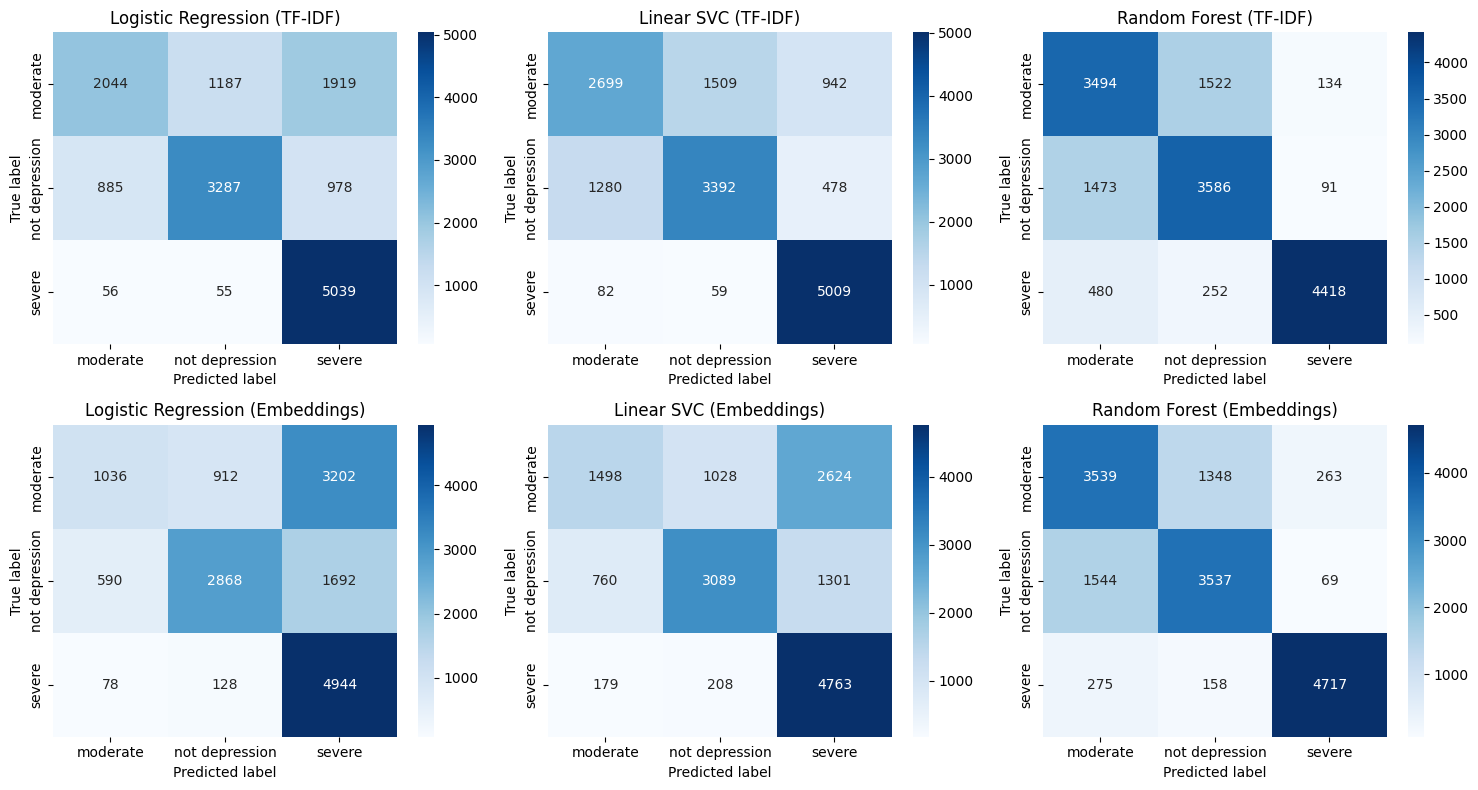
\includegraphics[width=0.8\linewidth]{img/confusion-matrices.png}
    \caption{Confusion Matrices}
    \label{Fig_2}
\end{figure}

\subsection{Deep Learning Models Results}

Table ~\ref{Table_3} displays the results of the BiLSTM models trained with two types of GloVe embeddings: general-domain and Twitter-specific. The BiLSTM model with Twitter-based embeddings slightly outperformed the general GloVe model in F1-score (62.4\% vs. 60.6\%) and precision (64.1\% vs. 62.8\%). This was expected, since domain-specific embeddings should better capture linguistic patterns of social media texts.

\begin{table}
    \centering
    \caption{BiLSTM Models Results}
    \label{Table_3}
    \begin{tabular}{ccccc}
        \toprule
            \textbf{Model}          & 
            \textbf{Accuracy (\%)}  & 
            \textbf{F1 Score (\%)}  & 
            \textbf{Recall (\%)}    & 
            \textbf{Precision (\%)} \\
        \midrule
            BiLSTM (General GloVe)  & 63.3 & 60.6 & 63.3 & 62.8 \\
            BiLSTM (Twitter GloVe)  & 61.4 & 62.4 & 61.4 & 64.1 \\
        \bottomrule
    \end{tabular}
\end{table}

However, both BiLSTM model variants underperformed heavily when compared to the top-performing traditional classifiers. While BiLSTM models may benefit from further hyperparameter tuning or additional data, these results show that their complexity did not translate to superior performance in this setting. I consider that this poor performance is largely due to the limited quality and quantity of the training data, particularly the low representation of severe cases. Moreover, the synonym-replacement data augmentation approach I used may have failed to introduce sufficient new context. For future work, I recommend exploring data augmentation methods based on transformer models like BERT, which can generate more contextually diverse samples.

\subsection{DistilBERT Fine-Tuning Results}

Finally, I evaluated a fine-tuned DistilBERT model using a two-stage training process involving masked language model pre-training followed by supervised classification fine-tuning. The evaluation metrics after 6 epochs are as follows: accuracy of 66.4\%, F1-score of 66.4\%, precision of 66.7\%, and recall of 66.4\%.

While DistilBERT did not outperform the Random Forest classifier with embeddings, it still achieved competitive results and performed better than both BiLSTM models. I attribute its relatively modest performance to similar factors affecting the BiLSTM models: limited quality and quantity of training data and heavy class imbalance. Additionally, unlike with the BiLSTM experiments, no data-level solutions such as augmentation or oversampling were applied here. Given that transformer-based models are more computationally expensive, with sufficient training time and resources, further fine-tuning and extended training could likely improve DistilBERT performance and help it surpass simpler ensemble methods.

In summary, the best performing model across all experiments was the Random Forest classifier trained on sentence embeddings, with an F1-score of 76.4\%. This was followed closely by the TF-IDF version of the same model and the DistilBERT classifier. Deep learning models using BiLSTM performed reasonably but failed to surpass simpler methods.

The confusion matrices reveal that most models struggled with correctly classifying the "severe" class due to its low representation in the dataset. However, augmentation techniques and class weighting helped alleviate this to some extent.
    \section{Conclusion}

In this project, I explored different methods: traditional machine learning, deep learning, and transformer-based models, to classify depression severity from social media text. My best results came from the Random Forest classifier using sentence embeddings, which outperformed both the BiLSTM and DistilBERT models.

I found that the limited size and quality of my dataset, especially the low number of severe cases, made the task challenging for all approaches. Although I used data augmentation, resampling and class weighting to help with class imbalance, these strategies only partially addressed the issue. I believe that more advanced augmentation techniques and larger, better-quality datasets are needed to improve performance, especially for deep learning and transformer models.

While my fine-tuned DistilBERT model performed competitively, it was more computationally demanding and did not surpass the simpler Random Forest in this setting. With more time and resources, further fine-tuning and training could lead to better results with transformer-based models.

Overall, my findings suggest that traditional and simple machine learning models with strong feature representations remain effective, especially when data and computational resources are limited. For future work, I recommend focusing on two points of research. First, more effort should be put into collecting high-quality and diverse datasets specific to this domain. Second, since depression should ideally become less prevalent over time, naturally occurring high-quality data for this task may be scarce. This makes it even more important to develop advanced data augmentation techniques and carefully fine-tune neural networks and transformer models to unlock their full potential.
    
    \bibliographystyle{splncs04}
    \bibliography{references}
\end{document}
